\documentclass{article}
\usepackage[utf8]{inputenc}
\usepackage{pdfpages}

\author{Accordi Gianmarco}
\title{Reverse Engineering}

\usepackage{natbib}
\usepackage{graphicx}
\usepackage{minted}
\usepackage{tabularx}
\usepackage{tikz}
\usepackage{pgfplots}
\usepackage{hyperref}

\usemintedstyle{fruity}
\date{}

\begin{document}

\maketitle

\section{Introduction}

\textbf{Reverse Engineering} is the process of understanding how system made by man is working, by looking at it an trying to reverse the operations it does in order to understand its behavior.
Its like a scientific research but in this case we are not interested in natural phenomenon.
This kind of process has been applied to a lot of different fields, from mechanical engineering to chemical engineering, so as the name suggested it is applied to all field of engineering: these are the fields in which we can take apart the work done by other human being and trying to understand how they have build such a system.
The necessity of this such an analysis of a system is usually required because creator of a system tends to disclose how they've built it, this mean that they obscure their work in order to protect their creators rights.
The purpose of this document is to give an introduction on \textbf{Reverse Engineering} specifically in the field of Software Engineering.
The process of Reverse Engineering applied to Software products can be done at any level of the production, but it usually involves two stages \footnote{\url{https://en.wikipedia.org/wiki/Reverse_engineering}}:
\begin{itemize}
    \item \textbf{Redocumentation}: since usually the given software product that we want to analyze is already compiled we want to be able to reach an higher level of abstraction to better understand the code;
    \item \textbf{Design Understanding}: once that we have been able to get an higher abstraction of our code we can use our capacity and knowledge in order to understand what the program does and how it does it, so we want to follow the development process of the creators of such code.
\end{itemize}
Disclose the design features can be understand with two approaches:
\begin{itemize} 
    \item \textbf{Dynamic Analysis}: this is an on the field approach, in which you launch the program and you register what the program is doing, and by analyzing the impact it has on the environment(print,systemcalls,...) you try to figure out what it does;
    \item \textbf{Static Analysis}: analyze the code without launch it, you analyze only the output you've obtained from the \underline{Redocumentation} part.
\end{itemize} 
In next sections we will analyze this approaches along with the stage involved in doing them.
Then we proceed in order to define which is the best strategy based on what we have seen. Finally an example is provided taken from a CTF. 

\subparagraph{Reverse Engineering in Software Engineering}
As previously stated this document focus its attention on Reverse Engineering applied to software. When a new software is released it is usually provided already compiled to the specific architecture, so you get the binary of this code.
The binary, as the name suggests, contains binary instructions that are targeted to be understood by a specific machine with a specific architecture, this means that it cannot be understand easily from a human being.
For the developers this is usually a wanted feature, since this make the reverse engineering process more difficult for other companies that wants to disclose their design features.
To be even more secure companies also rely on the usage of some \underline{Obfuscation Technique} that makes the reverse engineering process even harder. This leads to the development of new research fields focused on trying to remove obfuscation, also in an automate way \citep{1566145}.
Some techniques used for obfuscate binaries are Packing( in which the source code pack and unpack the .text section as long as it execute)\citep{SlidePackers}, Dynamic Code Mutation( in which the code mutate during execution), Code Generation( the program generates code during program execution) or by Binary Instumentation \cite{paperInstrumentation}.
So in the end software is usually not fully disclose for two main reasons: protection of intellectual property and malware. In next sections we will see different techniques that can be used in order to defeat make the process of reverse engineering more easy.

\clearpage

\section{Stages} 
The process of \textbf{Reverse Engineering} pass through 2 main stages, the \underline{Redocumentation} part analysis statically the executable starting from a decompilation process.
while the second part called \underline{Design Understanding} involves the outcome of the previous stage combined with dynamic analysis, based on the strategy we choose to adopt. 

\subsection{Redocumentation}
\label{section:redocumentation}
The program we get is usually a binary file so the first steps in order to get an higher level representation of it is to disassemble it.
\begin{figure}[htp]
    \centering
    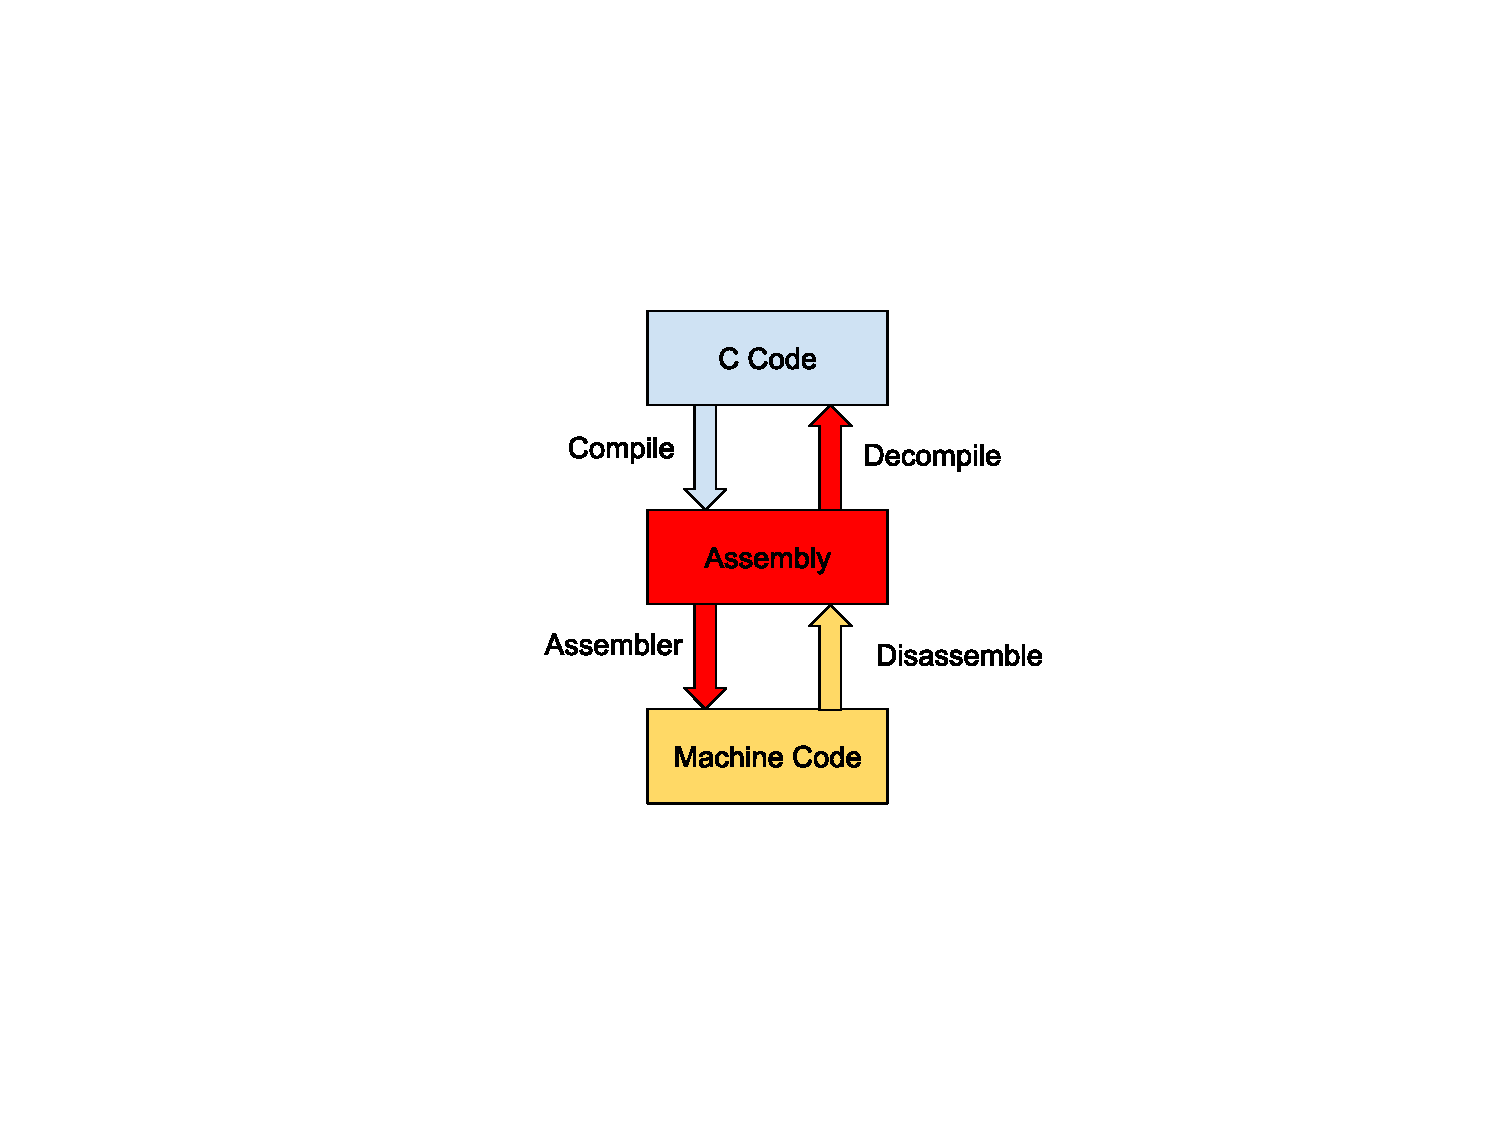
\includegraphics[width=1\textwidth]{images/redocumentation.pdf}
    \caption{Compilation and Decompilation steps \citep{SlideReverse}}
    \label{fig:redocumentation}
\end{figure}
Figure \ref{fig:redocumentation} refers to the case of compiled languages( and we will refers to the them from now on), as we can see when someone wants to make its code executable has to go throw a set of steps usually:
\begin{itemize}
    \item \textbf{Compilation}: from the high level code( say for example C code) you use the compiler \footnote{\url{https://en.wikipedia.org/wiki/Compiler}} to generate a low level language that usually is Assembly code;
    \item \textbf{Assembler}: in this stage you pass from Assembly code, that has an high correspondence with the machine code instructions so it is targeted to a specific architecture \footnote{\url{https://en.wikipedia.org/wiki/Assembly_language}}, into machine code that can be executed.
\end{itemize}
In fact what we usually have is the machine code, the executable file. From it we have to extract useful information to understand what it does, this again requires to revert the previous operations, as shown in \ref{fig:redocumentation}( going down to up):
\begin{itemize}
    \item \textbf{Disassemble}: from the machine code of a specific architecture(that can be x86-64 or arm) we get the correspondent Assembly code;
    \item \textbf{Decompile}: from the assembly code we have obtain our aim is to get the high level source code that has generate it as similar as possible to the original one.
\end{itemize}
The process of generating an executable is not an invertible function \footnote{\url{https://en.wikipedia.org/wiki/Decompiler}} This means that by doing so we lost some information, that makes the inverse process quite harder.
In fact the output of the decompilation stage can vary based on the compiler used to perform compilation and the presence of metadata present inside of the executable, if for example has been included debug information or if instead it has been stripped of all the metadata. The outcome of the compilation change also based on the optimization enabled at compile time.
As previously state some code can also be harder to be decompiled since it has been obfuscated with different techniques, another example is the insertion of instructions that doesn't change the flow of executed instructions but it insertion broke the alignment and so the decompiler is not able to recognize instructions in the correct way.
The \underline{output of the Disassemble stage} can be analyzed as shown in figure \ref{fig:decompilationoutput}. We can organize block of assembly instructions inside block that are executed sequentially, until some instruction that controls the execution flow are encountered, like jump instruction.
In such cases the flow is divided into different block of other assembly instructions.
\begin{figure}[htp]
    \centering
    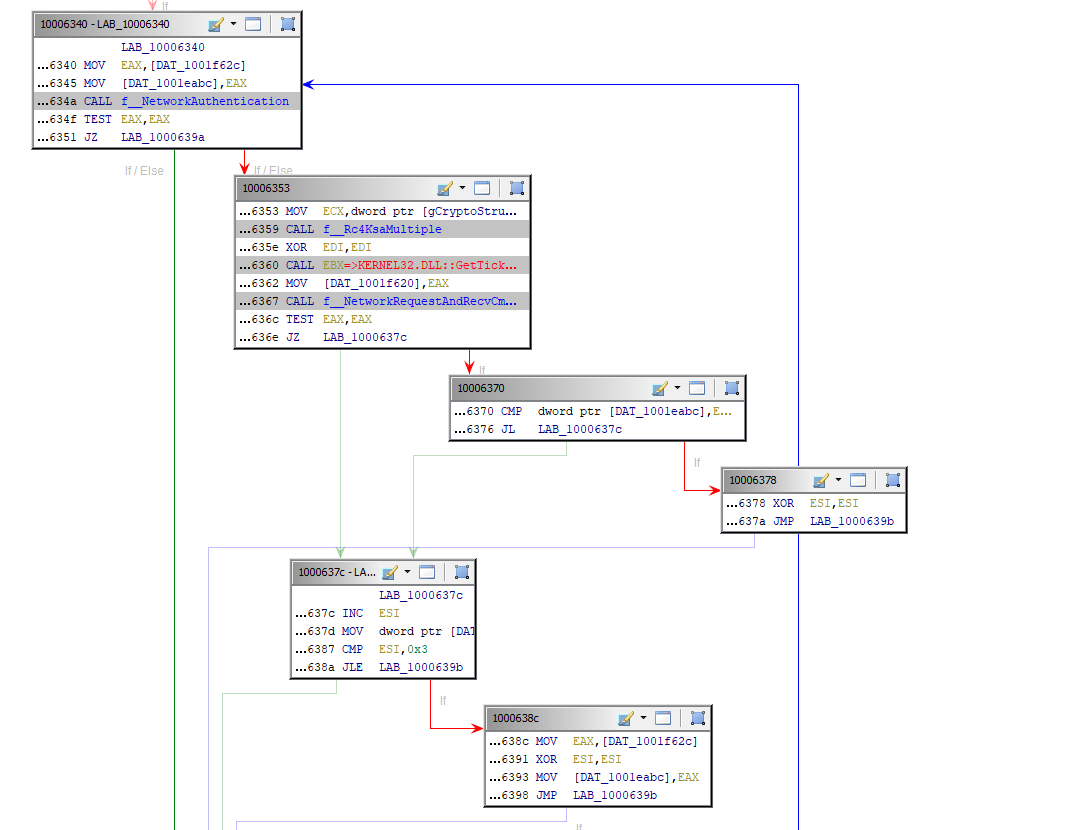
\includegraphics[width=1\textwidth]{images/graphview.png}
    \caption{Analysis of the Decompilation's output stage.}
    \label{fig:decompilationoutput}
\end{figure}
The output of the Decompilation part can be read mode easily since it will be something similar to the original source code that has produced the executable file. 
\begin{figure}[htp]
    \centering
    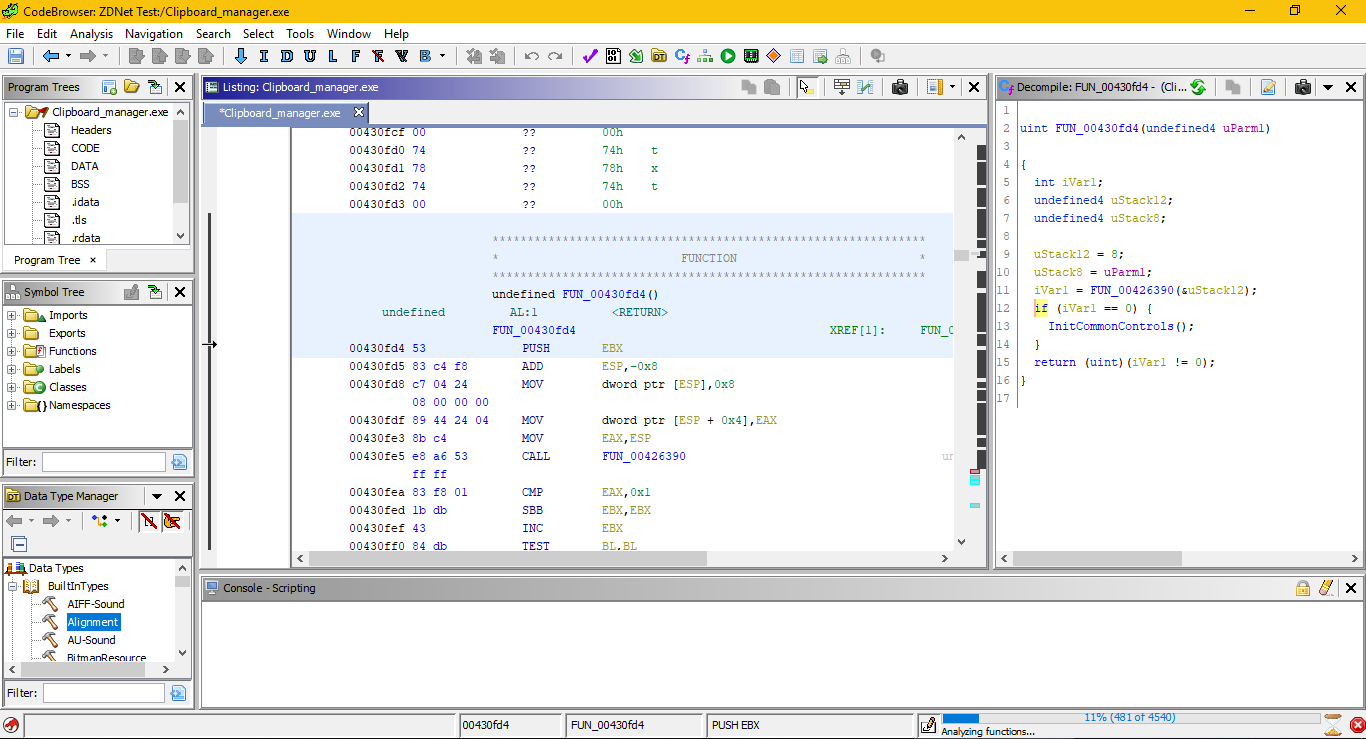
\includegraphics[width=1\textwidth]{images/ghidra.png}
    \caption{Ghidra GUI after analyzing an executable file.}
    \label{fig:ghidraoutput}
\end{figure}
Different tools exists that allows to perform decompilation of an executable. Most famous one are \textit{Ghidra} and \textit{IDA Pro}. Figure \ref{fig:ghidraoutput} show an example output of Ghidra. The reference of supported architecture for decompilation can be found here \footnote{\url{https://en.wikipedia.org/wiki/Ghidra}}.
Ghidra makes use of automated tools that helps in generating the source code starting from the executable. From interface we can look at the whole space of the object file: from the address of the library, to the assembly code, to the constant variables loaded inside the file.
The readability of the output depends on the quality of the tool used to decompile and on the present metadata, but it is more than recommended a user inspection of code, for example to better understand the type of the variable.
\begin{figure}[htp]
    \centering
    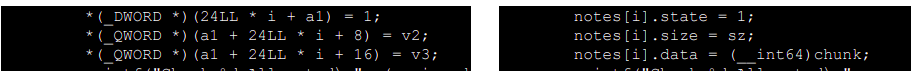
\includegraphics[width=1\textwidth]{images/coderead.png}
    \caption{Code readability after inspection of the struct.}
    \label{fig:coderead}
\end{figure}
As you can see in image \ref{fig:coderead} the code on the right is more readable after inspection if the code, and the definition of a strut hat better fits the memory structure that is used by the executable.
Up to know we have assumed to have under analysis an executable from a \textit{Compiled Language}, but the same things can be applied to \textit{Interpreted Language} \footnote{\url{https://en.wikipedia.org/wiki/Compiled_language}} like for example Java, in which some tool exists in order to analysis the bytecode produced by java \footnote{\url{http://java-decompiler.github.io/}}.
The work done during this stage is important in the first strategy that we will purse in order to discover design features of the programs under analysis: \underline{Static Analysis}.

\clearpage

\subsection{Design Understanding}
The objective of the Reverse Engineering task is to understand the \textit{Design Features} of the program under analysis. So in order to reach this results one can use different techniques, that can be generalized into two main categories: \textbf{Static Analysis} and \textbf{Dynamic Analysis}.

\paragraph{Static Analysis}
What we have seen during the \textit{Redocumentation} stage \ref{section:redocumentation} is what we can think as Static analysis, in fact it is the process of code analysis without regard of its execution or input \citep{LessonReverse}.
From this analysis we can take a look at the:
\begin{itemize}
    \item \textbf{Control flow}: the code is broke down into block, that merged together instructions that will be executed sequentially, this separation in block can be done by looking at how the control instructions are placed, like if or while loop \ref{fig:decompilationoutput}, in this way we can try to understand which is the path block executed by the program sequentially, so we can follow the execution flow;
    \item \textbf{Data Flow}: helps in understanding how the data flows inside the program, from the input we can give to the program to the final outcome of its execution.
\end{itemize}

\paragraph{Dynamic Analysis}
Opposed to Static the Dynamic Analysis instead rely on the execution of the program regarding on the input provided to it. In this case we try to launch the executable with different inputs and look at the different outcome we got.
\begin{figure}[htp]
    \centering
    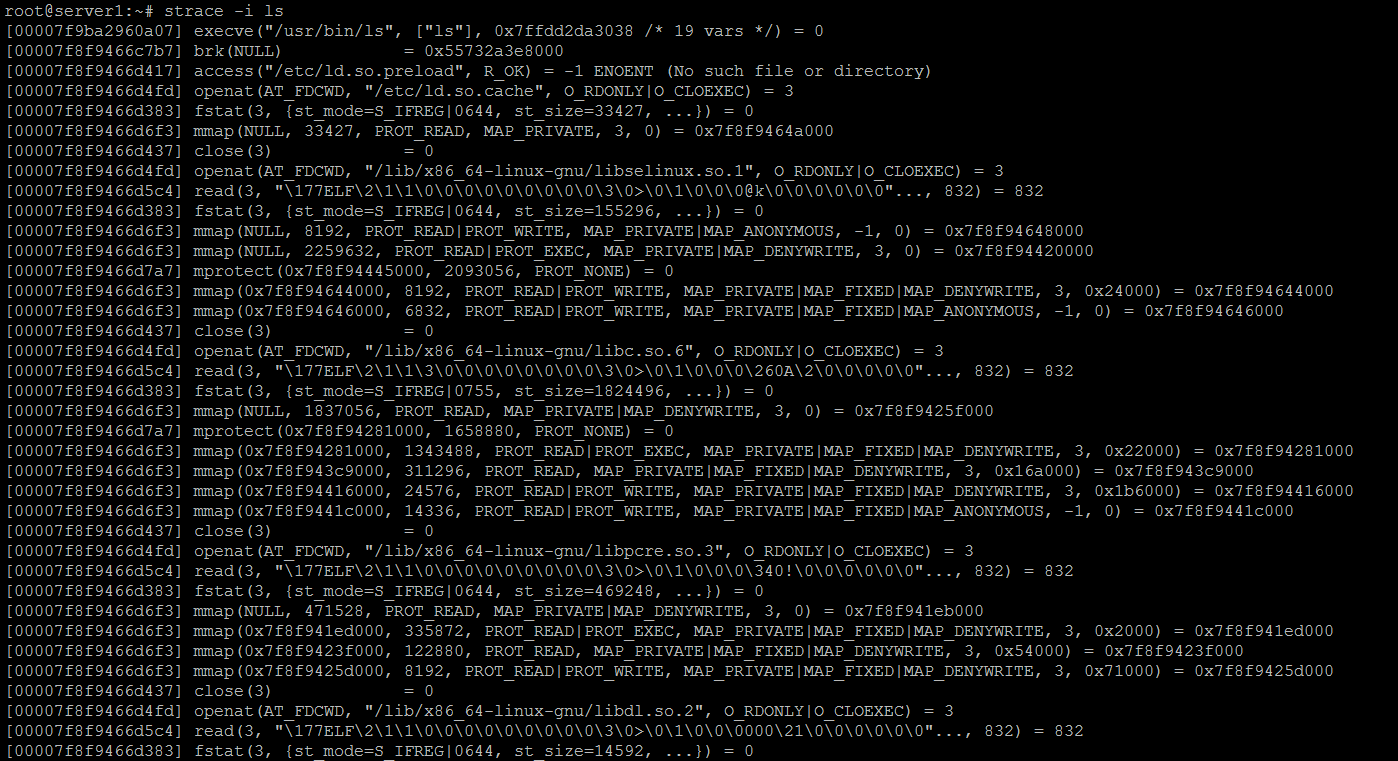
\includegraphics[width=1\textwidth]{images/strace.png}
    \caption{The output of an analysis with strace}
    \label{fig:strace}
\end{figure}
And by looking at the output returned by the executable we try to guess what the program does. We can also use some other tools to understand what the executable does by looking at the system calls invocation done by it, in this case we can user \textit{strace}\footnote{\url{https://en.wikipedia.org/wiki/Strace}}. As we can see in figure \ref{fig:strace} the output will make a summary of the various system calls done by a certain program.
\textit{Strace} allows to analysis how the executable access to the privileged kernel mode, how the program switch its execution from user mode to kernel mode. Other tools that can be used are \textit{ltrace} and \textit{ptrace}. In general you can look to the access made by the program to the disk memory, to the network usage of the program, etc\dots.
\begin{figure}[htp]
    \centering
    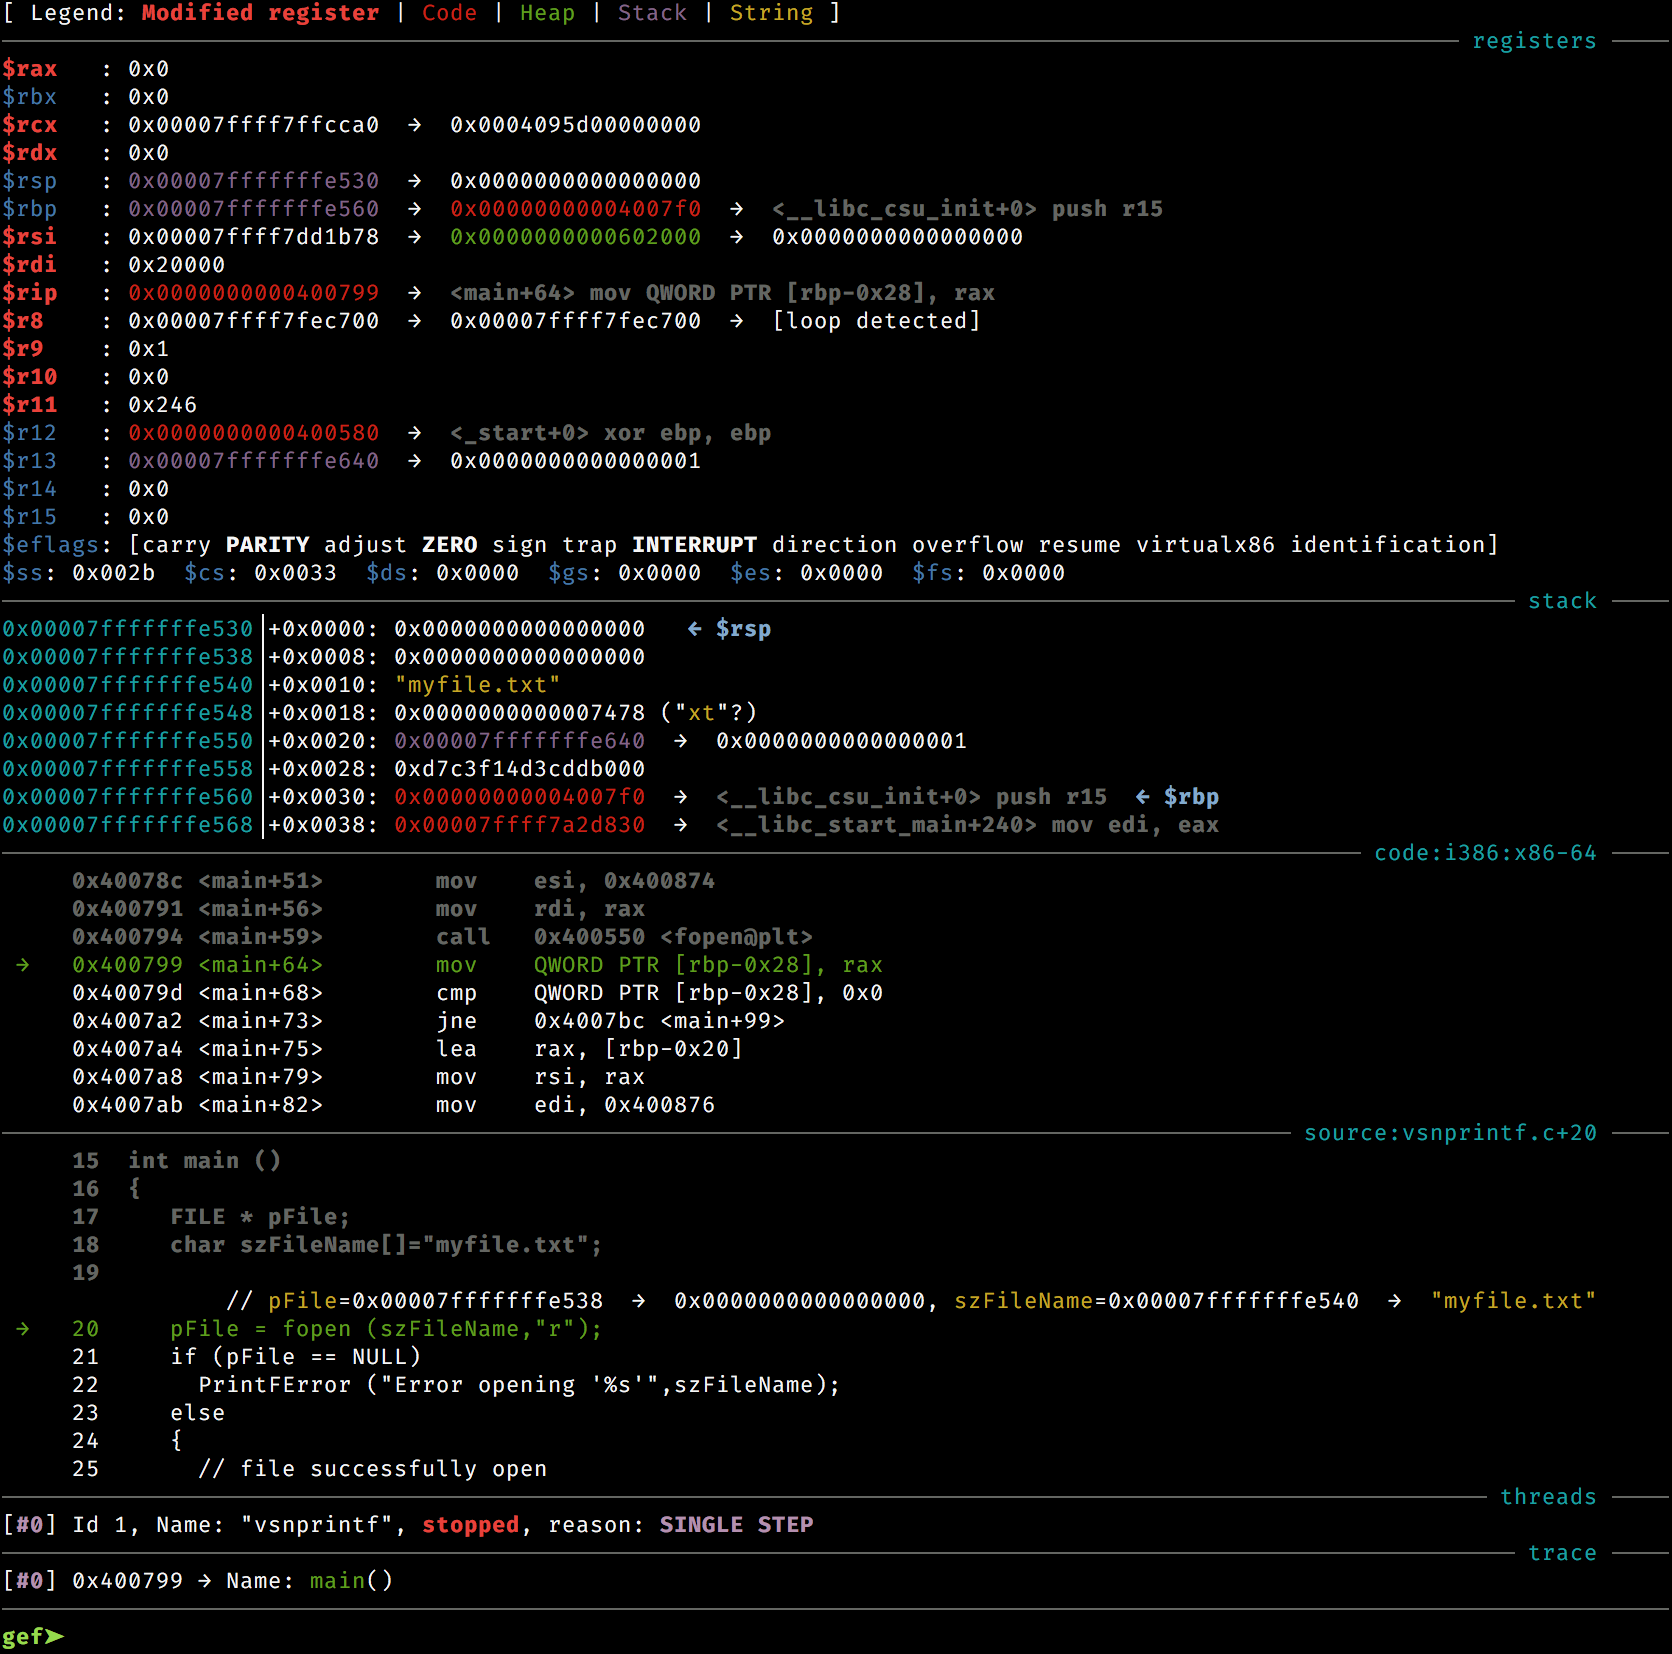
\includegraphics[width=1\textwidth]{images/gdb.png}
    \caption{The output of GDB during a program execution.}
    \label{fig:gdb}
\end{figure}
Another example of a useful tool that can be used during Dynamic Analysis we have to be able to analyze the behavior of the program as long as it is executing: in this case we can take advantage of \textit{Debbuger}, that permits to execute an executable in a controlled environment in which we are able to follow the progress of the program\footnote{\url{https://en.wikipedia.org/wiki/Debugger}}. By using breakpoints to stop executions, we can find out the code that is actually executed by the program, and also take a look and modify the content of the registers.
Image \ref{fig:gdb} shows an example of a well known and used debugger: \textit{GDB}. It is quite used debugger that works for different programming languages like C, C++, Pascal, Fortran, etc\dots.
The image shows an example of its usage after hitting a breakpoint: GDB shows the content of the registers and at which line in the assembly code the execution of the program has reached. You can for example use GDB in order to create a dump of the memory that you can better analyze with want we have seen in \ref{section:redocumentation} to better understand whats happening.
Note that \ref{fig:gdb} shows also to which line of the source code the assembly line corresponds. Obviously this will not be possible in most of the case when doing Reverse Engineering, since who has made the executable want to make our job harder.

\subsection{Which is the best strategy to adopt?}
\begin{figure}[htp]
    \centering
    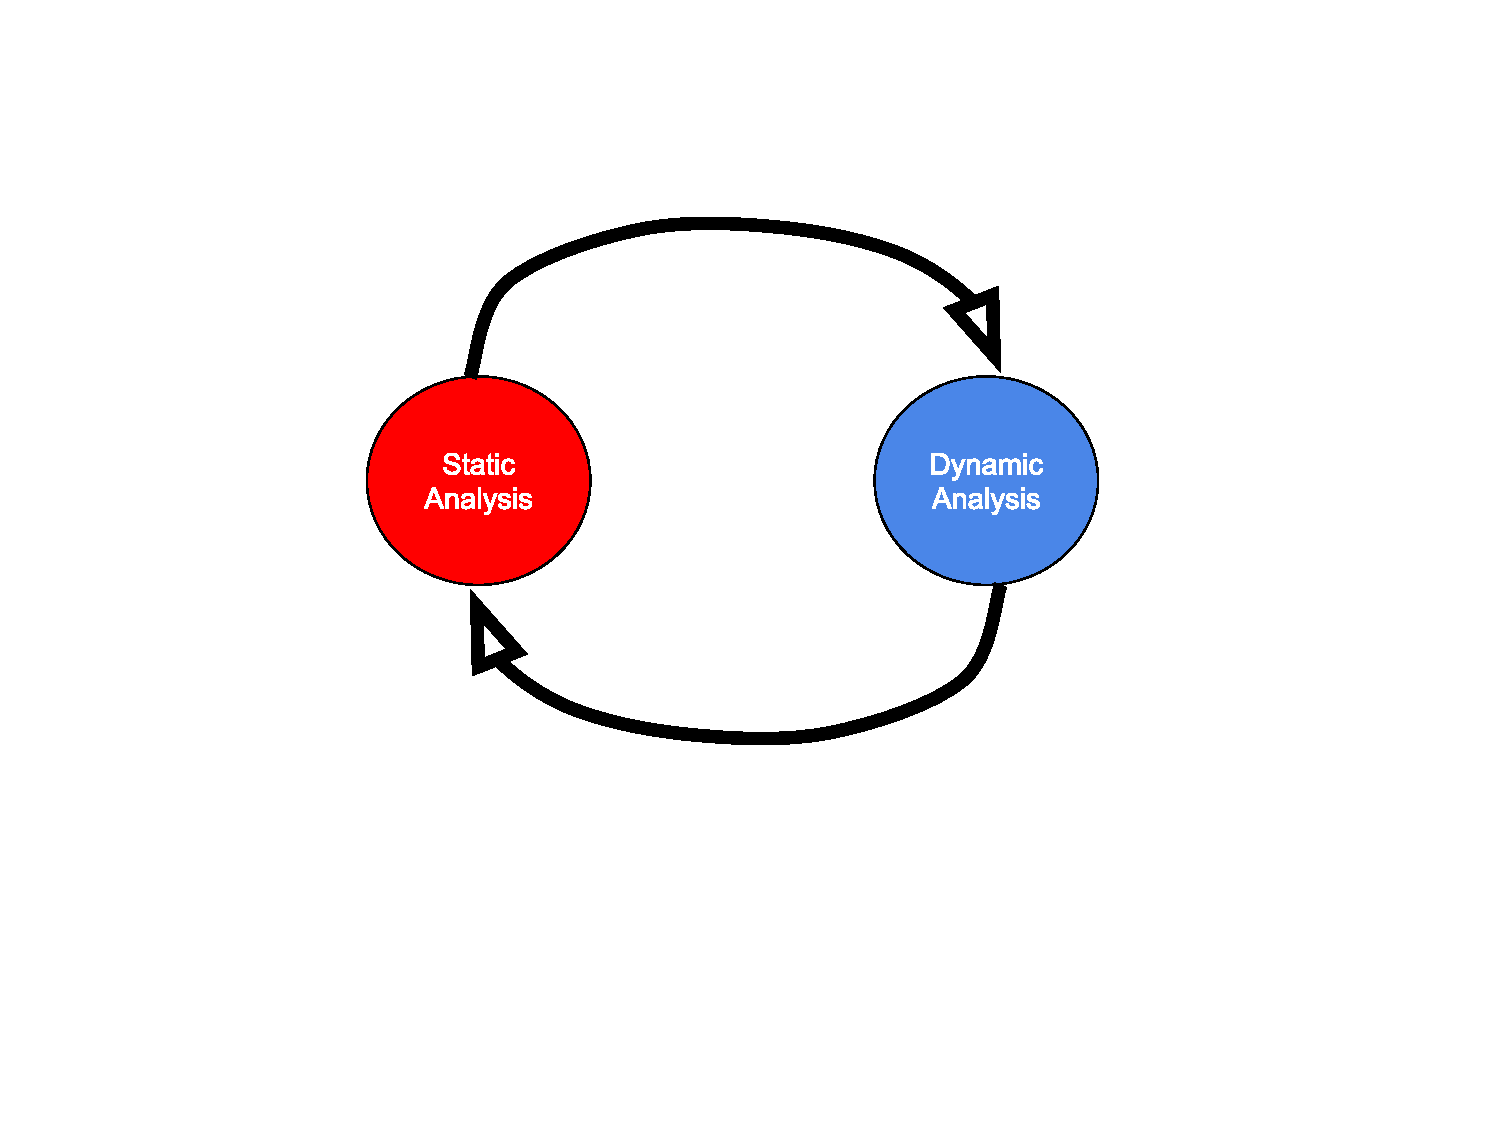
\includegraphics[width=1\textwidth]{images/staticAndDynamic.pdf}
    \caption{Relationship among Static and Dynamic Analysis.}
    \label{fig:gdb}
\end{figure}
One can wonder which approach should choose among the two we have seen: if the best idea is to use \textit{Dynamic} or \textit{Static} analysis. Both have disadvantages and advantages: for example static analysis allows to reach an higher code coverage, but if the analyzed software use some obfuscation technique it may be the case that some behavior is shown only during the execution of the program( is the case of packer\citep{packer}).
But dynamic analysis has a low code coverage, and so some details in the behavior of a program can be missed by a dynamic analysis.
All of this to highlight how the best approach to use is to use both of them in combination, doing static analysis while also doing dynamic analysis, based on the situation we are dealing with. 
So you need to adapt you approach regarding to the software you are approaching to analyze, as we should see in the next example.

\clearpage

\section{keycheck\_baby}
In this section we will cover how someone can approach a real example, that in this case is the \textit{keycheck\_baby} CTF.
In order to decide which approach we should use we can execute try to analyze the header of the file under analysis with the command as in:
\begin{minted}[linenos, bgcolor=white, escapeinside=!!]{bash}
    $ file keycheck_baby
\end{minted}
In our case as output you will get
\begin{minted}[linenos, bgcolor=white, escapeinside=!!]{bash}
    keycheck_baby: ELF 64-bit LSB shared object, x86-64, version 1 (SYSV), dynamically linked, interpreter /lib64/ld-linux-x86-64.so.2, BuildID[sha1]=7c050cd827cea1dfa736ac05bbac7b343fbf1d01, for GNU/Linux 3.2.0, not stripped
\end{minted}
The important part here is that the executable is \textit{not stripped}\footnote{\url{https://en.wikipedia.org/wiki/Stripped_binary}}, this means that the executable contains also debug information that can be used both by a debugger but it also helps during the decompilation process.
Other important information can be returned by running the following command:
\begin{minted}[linenos, bgcolor=white, escapeinside=!!]{bash}
    $ checksec keycheck_baby
\end{minted}
Which gives as output:
\begin{minted}[linenos, bgcolor=white, escapeinside=!!]{bash}
    Arch:     amd64-64-little
    RELRO:    Partial RELRO
    Stack:    Canary found
    NX:       NX enabled
    PIE:      PIE enabled
\end{minted}
Partial RELRO means that only small parts of the GOT and PLT are writable, while a canary aims in avoiding canaries. NX enabled makes the stack not executable and PIE allows the code to be relocatable in case ASLR is active.
The next step is to start a decompilator to try and analyze the decompiled executable. In our case we will use Ghidra. Ghidra will analyze the executable, and then we can look at the output of the disassemble and decompilation.
First we need to find the entry point of the execution that can be easily found by searching inside the \textit{Symbol Tree} the \textit{main}, in order to a reconstruction of the source code:
\begin{figure}[htp]
    \centering
    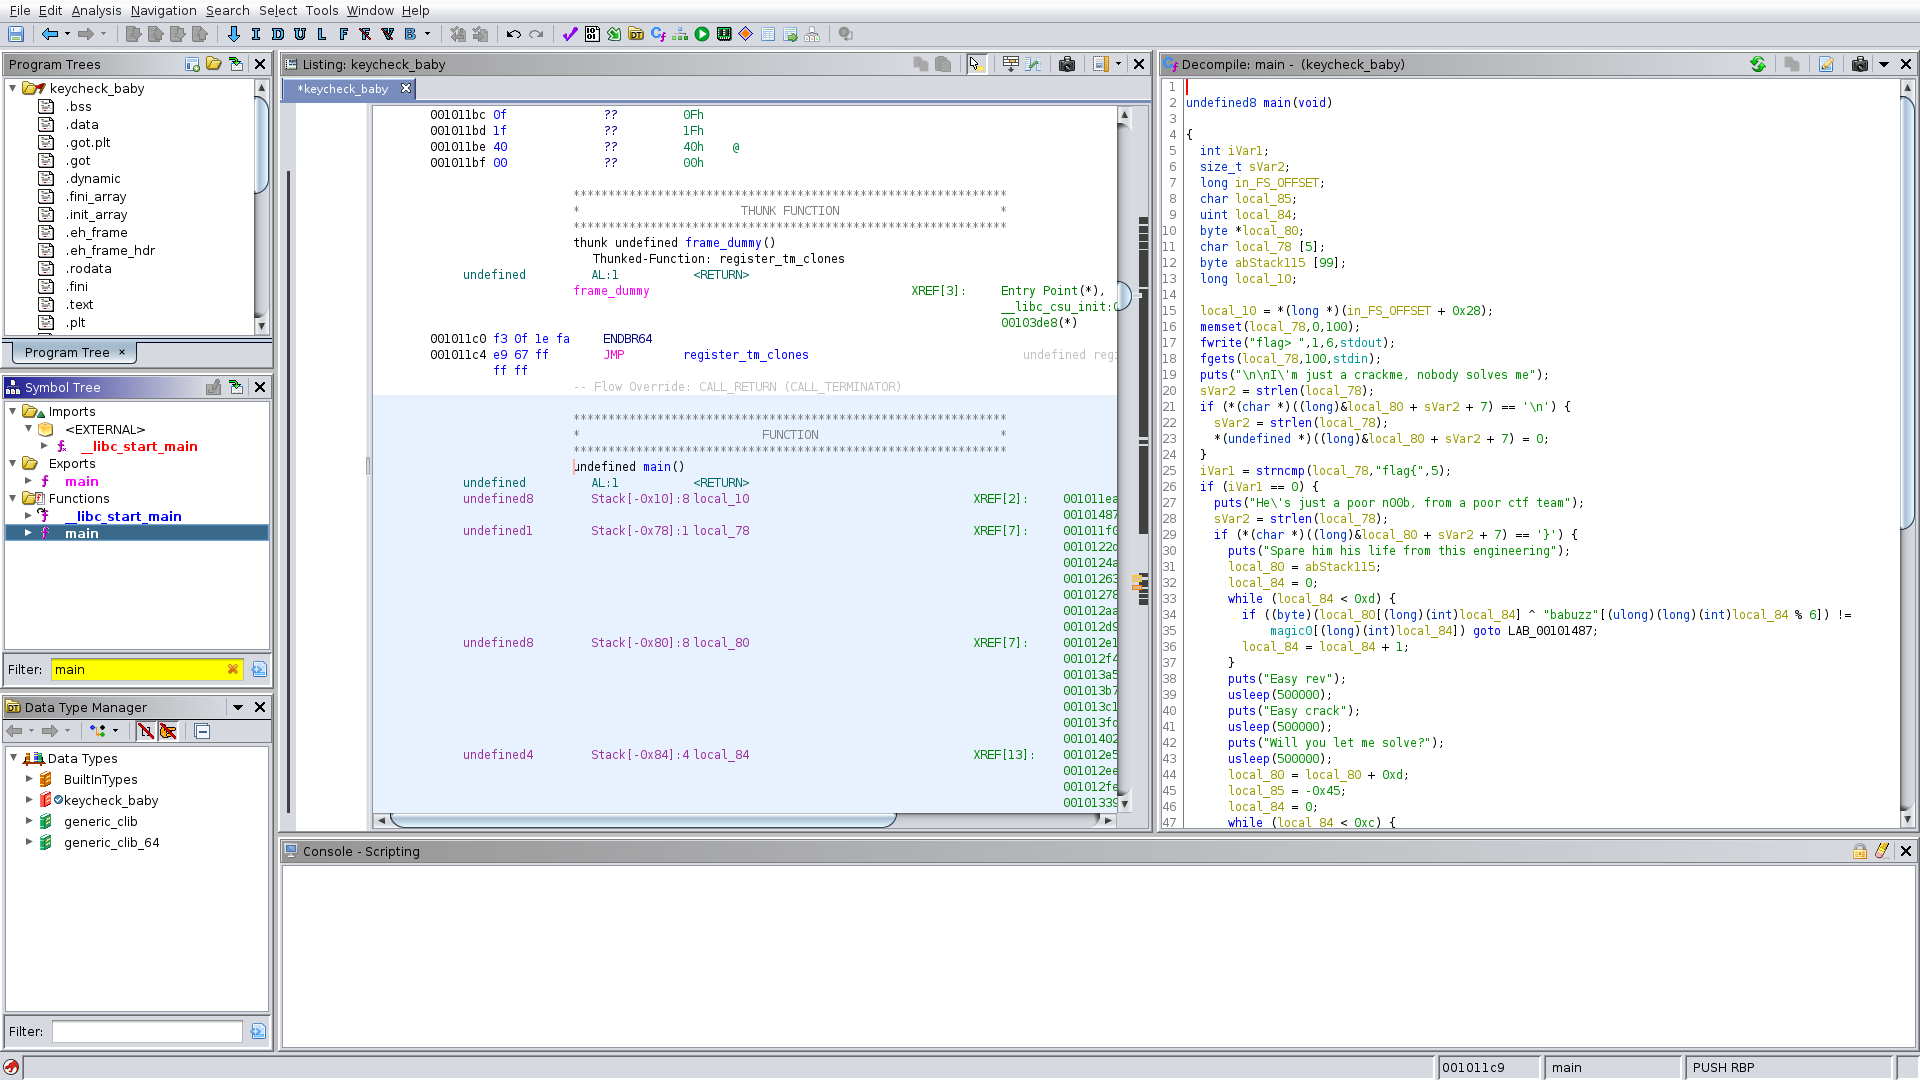
\includegraphics[width=1\textwidth]{images/ghidrakeycheck.png}
    \caption{The output of GDB after analyzing the keycheck executable.}
    \label{fig:keycheckgdb}
\end{figure}
By taking a look a the code we can see that no obfuscation technique has been used since the whole code is there: so we can use as an approach static analysis, because there aren't some part that are crypted, and there isn't no code that is used to generate other code, in that case we should have used dynamic analysis
in order to look at the code during execution or in order to do a dump file of the memory.
As we have seen in \ref{fig:coderead} in order to make things easier is a good idea to check if we can improve the code readability by retyping variable and assign a different name to them.
For example by saying that the input of the \textit{memset} function is a \textit{char *} in our case.
Now we will take a look at the most important part of the code.
This first part will take as input the flag and it will store it inside the \textit{input} variable. It checks that the string terminate with the string terminator.
At the next step the input is compared with the \textit{flag\{} string:
\begin{minted}[linenos, bgcolor=black, escapeinside=!!]{c}
  iVar1 = strncmp(input,"flag{",5);
  if (iVar1 == 0) {
    puts("He\'s just a poor n00b, from a poor ctf team");
    sVar2 = strlen(input);
    if (*(char *)((long)&input + sVar2) == '}') {
\end{minted}
and also verifies that the flag ends with a \textit{\}}.
Now the program checks the first 0xd(13) characters of the input string, by accessing it with the \textit{index}. And it checks that the value of the input string at index elevated
at the casted int value of the relative character present in the \textit{babuzz} string at position index % 6. 
\begin{minted}[linenos, bgcolor=black, escapeinside=!!]{c}
    index = 0;
    while (index < 0xd) {
        if ((byte)(input[(long)(int)index] ^ "babuzz"[(ulong)(long)(int)index % 6]) !=
            magic0[(long)(int)index]) goto LAB_00101487;
        index = index + 1;
    }
\end{minted}
If this is not the case the flow of execution jumps at the end of the code at the label \textit{LAB\_00101487} before checking the canary.
\begin{minted}[linenos, bgcolor=black, escapeinside=!!]{c}
    LAB_00101487:
    if (local_10 == *(long *)(in_FS_OFFSET + 0x28)) {
        return 0;
    }
\end{minted}
//TODO



\subsection{Example of code}
Here you can fine an example of how to add some code. It is using the package minted with basic option enabled.
You can write code in place:
\begin{minted}[linenos, bgcolor=black, escapeinside=!!]{python}
import numpy as np
    
def incmatrix(genl1,genl2):
    m = len(genl1)
    n = len(genl2) !\label{myline}!
    M = None #to become the incidence matrix
    VT = np.zeros((n*m,1), int)  #dummy variable
    
    #compute the bitwise xor matrix
    M1 = bitxormatrix(genl1)
    M2 = np.triu(bitxormatrix(genl2),1) 
...
\end{minted}
You can reference to a line
The important line is line \ref{myline}.

You can use an external file and ave the code as listing.
\begin{listing}[ht]
\inputminted[linenos, bgcolor=black, escapeinside=!!]{python}{x.py}
\caption{Example from external file}
\label{listing:3}
\end{listing}
 
The important line is line \ref{anotherline} of Listing~\ref{listing:3}.

\section{Conclusion}


\bibliographystyle{plain}
\bibliography{references}
\end{document}
